\documentclass[12pt,a4paper,twoside,openright]{report}
\let\openright=\cleardoublepage



%%% Choose a language %%%

\newif\ifEN
\ENtrue   % uncomment this for english
%\ENfalse   % uncomment this for czech

%%% Configuration of the title page %%%

\def\ThesisTitleStyle{mff} % MFF style
%\def\ThesisTitleStyle{cuni} % uncomment for old-style with cuni.cz logo
%\def\ThesisTitleStyle{natur} % uncomment for nature faculty logo

\def\UKFaculty{Faculty of Mathematics and Physics}
%\def\UKFaculty{Faculty of Science}

\def\UKName{Charles University in Prague} % this is not used in the "mff" style

% Thesis type names, as used in several places in the title
\def\ThesisTypeTitle{\ifEN BACHELOR THESIS \else BAKALÁŘSKÁ PRÁCE \fi}
%\def\ThesisTypeTitle{\ifEN MASTER THESIS \else DIPLOMOVÁ PRÁCE \fi}
%\def\ThesisTypeTitle{\ifEN RIGOROUS THESIS \else RIGORÓZNÍ PRÁCE \fi}
%\def\ThesisTypeTitle{\ifEN DOCTORAL THESIS \else DISERTAČNÍ PRÁCE \fi}
\def\ThesisGenitive{\ifEN bachelor \else bakalářské \fi}
%\def\ThesisGenitive{\ifEN master \else diplomové \fi}
%\def\ThesisGenitive{\ifEN rigorous \else rigorózní \fi}
%\def\ThesisGenitive{\ifEN doctoral \else disertační \fi}
\def\ThesisAccusative{\ifEN bachelor \else bakalářskou \fi}
%\def\ThesisAccusative{\ifEN master \else diplomovou \fi}
%\def\ThesisAccusative{\ifEN rigorous \else rigorózní \fi}
%\def\ThesisAccusative{\ifEN doctoral \else disertační \fi}



%%% Fill in your details %%%

% (Note: \xxx is a "ToDo label" which makes the unfilled visible. Remove it.)
\def\ThesisTitle{\xxx{Thesis title}}
\def\ThesisAuthor{\xxx{Your Name Surname}}
\def\YearSubmitted{\xxx{YEAR}}

% department assigned to the thesis
\def\Department{\xxx{Name of the department}}
% Is it a department (katedra), or an institute (ústav)?
\def\DeptType{\xxx{Department}}

\def\Supervisor{\xxx{Supername Supersurname}}
\def\SupervisorsDepartment{\xxx{department}}

% Study programme and specialization
\def\StudyProgramme{\xxx{study programme}}
\def\StudyBranch{\xxx{study branch}}

\def\Dedication{%
Dedication. \xxx{It is nice to say thanks to supervisors, friends, family, book authors and food providers.}
}

\def\AbstractEN{%
\xxx{Abstracts are an abstract form of art. Use the most precise, shortest sentences that state what problem the thesis addresses, how it is approached, pinpoint the exact result achieved, and describe the applications and significance of the results. Highlight anything novel that was discovered or improved by the thesis. Maximum length is 200 words, but try to fit into 120. Abstracts are often used for deciding if a reviewer will be suitable for the thesis; a well-written abstract thus increases the probability of getting a reviewer who will like the thesis.}
% ABSTRACT IS NOT A COPY OF YOUR THESIS ASSIGNMENT!
}

\def\AbstractCS{%
\xxx{You will need to submit both Czech and English abstract to the SIS, no matter what language you use in the thesis. If writing in English, translate the contents of \texttt{\textbackslash{}AbstractEN} into this field. In case you do not speak czech, your supervisor should be able to help you with the translation.}
}

% 3 to 5 keywords (recommended), each enclosed in curly braces.
% Keywords are useful for indexing and searching for the theses by topic.
\def\Keywords{%
\xxx{{key} {words}}
}

% If your abstracts are long and do not fit in the infopage, you can make the
% fonts a bit smaller by this setting. (Also, you should try to compress your abstract more.)
% Alternatively, consider increasing the size of the page by uncommenting the
% geometry modification in thesis.tex.
\def\InfoPageFont{}
%\def\InfoPageFont{\small}  %uncomment to decrease font size

\ifEN\relax\else
% If you are writing a czech thesis, you additionally need to fill in the
% english translation of the metadata here!
\def\ThesisTitleEN{\xxx{Thesis title in English}}
\def\DepartmentEN{\xxx{Name of the department in English}}
\def\DeptTypeEN{\xxx{Department}}
\def\SupervisorsDepartmentEN{\xxx{Superdepartment}}
\def\StudyProgrammeEN{\xxx{study programme}}
\def\StudyBranchEN{\xxx{study branch}}
\def\KeywordsEN{%
\xxx{{key} {words}}
}
\fi


\usepackage[a-2u]{pdfx}

\ifEN\else\usepackage[czech,shorthands=off]{babel}\fi
\usepackage[utf8]{inputenc}
\usepackage[T1]{fontenc}

% See https://en.wikipedia.org/wiki/Canons_of_page_construction before
% modifying the size of printable area. LaTeX defaults are great.
% If you feel it would help anything, you can enlarge the printable area a bit:
%\usepackage[textwidth=390pt,textheight=630pt]{geometry}
% The official recommendation expands the area quite a bit (looks pretty harsh):
%\usepackage[textwidth=145mm,textheight=247mm]{geometry}

%%% FONTS %%%
\usepackage{lmodern} % TeX "original" (this sets up the latin mono)

% Optionally choose an override for the main font for typesetting:
\usepackage[mono=false]{libertinus} % popular for comp-sci (ACM uses this)
%\usepackage{tgschola} % Schoolbook-like (gives a bit of historic feel)
%\usepackage[scale=0.96]{tgpagella} % Palladio-like (popular in formal logic).
% IBM Plex font suite is nice but requires us to fine-tune the sizes, also note
% that it does not directly support small caps (\textsc) and requires lualatex:
%\usepackage[usefilenames,RM={Scale=0.88},SS={Scale=0.88},SScon={Scale=0.88},TT={Scale=0.88},DefaultFeatures={Ligatures=Common}]{plex-otf}

% Optionally, choose a custom sans-serif fonts (e.g. for figures and tables).
% Default sans-serif font is usually Latin Modern Sans. Some font packages
% (e.g. libertinus) replace that with a better matching sans-serif font.
%\usepackage{tgheros} % recommended and very readable (Helvetica-like)
%\usepackage{FiraSans} % looks great
% DO NOT typeset the main text in sans-serif font!
% The serifs make the text easily readable on the paper.


% IMPORTANT FONT NOTE: Some fonts require additional PDF/A conversion using
% the pdfa.sh script. These currently include only 'tgpagella'; but various
% other fonts from the texlive distribution need that too (mainly the Droid
% font family).


% some useful packages
\usepackage{microtype}
\usepackage{amsmath,amsfonts,amsthm,bm}
\usepackage{graphicx}
\usepackage{xcolor}
\usepackage{booktabs}
\usepackage{caption}
\usepackage{floatrow}

% load bibliography tools
\usepackage[backend=bibtex,natbib,style=numeric,sorting=none]{biblatex}
% alternative with alphanumeric citations (more informative than numbers):
%\usepackage[backend=bibtex,natbib,style=alphabetic]{biblatex}
%
% alternatives that conform to iso690
% (iso690 is not formally required on MFF, but may help elsewhere):
%\usepackage[backend=bibtex,natbib,style=iso-numeric,sorting=none]{biblatex}
%\usepackage[backend=bibtex,natbib,style=iso-alphabetic]{biblatex}
%
% additional option choices:
%  - add `giveninits=true` to typeset "E. A. Poe" instead of full Edgar Allan
%  - `terseinits=true` additionaly shortens it to nature-like "Poe EA"
%  - add `maxnames=10` to limit (or loosen) the maximum number of authors in
%    bibliography entry before shortening to `et al.` (useful when referring to
%    book collections that may have hundreds of authors)
%  - for additional flexibility (e.g. multiple reference sections, etc.),
%    remove `backend=bibtex` and compile with `biber` instead of `bibtex` (see
%    Makefile)
%  - `sorting=none` causes the bibliography list to be ordered by the order of
%    citation as they appear in the text, which is usually the desired behavior
%    with numeric citations. Additionally you can use a style like
%    `numeric-comp` that compresses the long lists of citations such as
%    [1,2,3,4,5,6,7,8] to simpler [1--8]. This is especially useful if you plan
%    to add tremendous amounts of citations, as usual in life sciences and
%    bioinformatics.
%  - if you don't like the "In:" appearing in the bibliography, use the
%    extended style (`ext-numeric` or `ext-alphabetic`), and add option
%    `articlein=false`.
%
% possibly reverse the names of the authors with the default styles:
%\DeclareNameAlias{default}{family-given}

% load the file with bibliography entries
\addbibresource{refs}

% remove this if you won't use fancy verbatim environments
\usepackage{fancyvrb}

% remove this if you won't typeset TikZ graphics
\usepackage{tikz}
\usetikzlibrary{positioning} %add libraries as needed (shapes, decorations, ...)

% remove this if you won't typeset any pseudocode
\usepackage{algpseudocode}
\usepackage{algorithm}

% remove this if you won't list any source code
\usepackage{listings}


\hypersetup{unicode}
\hypersetup{breaklinks=true}

\usepackage[noabbrev]{cleveref}


% various forms of TODOs (you should remove this before submitting)
\usepackage[textsize=tiny, backgroundcolor=yellow!25, linecolor=black!25]{todonotes}
\newcommand{\xxx}[1]{\textcolor{red!}{#1}}

 % remove this before compiling the final version


% use this for typesetting a chapter without a number, e.g. intro and outro
\def\chapwithtoc#1{\chapter*{#1}\addcontentsline{toc}{chapter}{#1}}

% If there is a line/figure overflowing into page margin, this will make the
% problem evident by drawing a thick black line at the overflowing spot. You
% should not disable this.
\overfullrule=3mm

% The maximum stretching of a space. Increasing this makes the text a bit more
% sloppy, but may prevent the overflows by moving words to next line.
\emergencystretch=1em

\ifEN
\theoremstyle{plain}
\newtheorem{thm}{Theorem}
\newtheorem{lemma}[thm]{Lemma}
\newtheorem{claim}[thm]{Claim}
\newtheorem{defn}{Definition}
\theoremstyle{remark}
\newtheorem*{cor}{Corollary}
\else
\theoremstyle{plain}
\newtheorem{thm}{Věta}
\newtheorem{lemma}{Lemma}
\newtheorem{claim}{Tvrzení}
\newtheorem{defn}{Definice}
\theoremstyle{remark}
\newtheorem*{cor}{Důsledek}
\fi

\newenvironment{myproof}{
  \par\medskip\noindent
  \textit{\ifEN Proof \else Důkaz \fi}.
}{
\newline
\rightline{$\qedsymbol$}
}

% real/natural numbers
\newcommand{\R}{\mathbb{R}}
\newcommand{\N}{\mathbb{N}}

% asymptotic complexity
\newcommand{\asy}[1]{\mathcal{O}(#1)}

% listings and default lstlisting config (remove if unused)
\DeclareNewFloatType{listing}{}
\floatsetup[listing]{style=ruled}

\DeclareCaptionStyle{thesis}{style=base,font={small,sf},labelfont=bf,labelsep=quad}
\captionsetup{style=thesis}
\captionsetup[algorithm]{style=thesis,singlelinecheck=off}
\captionsetup[listing]{style=thesis,singlelinecheck=off}

% Customization of algorithmic environment (comment style)
\renewcommand{\algorithmiccomment}[1]{\textcolor{black!25}{\dotfill\sffamily\itshape#1}}

% Uncomment for table captions on top. This is sometimes recommended by the
% style guide, and even required for some publication types.
%\floatsetup[table]{capposition=top}
%
% (Opinionated rant:) Captions on top are not "compatible" with the general
% guideline that the tables should be formatted to be quickly visually
% comprehensible and *beautiful* in general (like figures), and that the table
% "head" row (with column names) should alone communicate most of the content
% and interpretation of the table. If you just need to show a long boring list
% of numbers (because you have to), either put some effort into showing the
% data in an attractive figure-table, or move the data to an attachment and
% refer to it, so that the boredom does not impact the main text flow.
%
% You can make the top-captions look much less ugly by aligning the widths of
% the caption and the table, with setting `framefit=yes`, as shown below.  This
% additionally requires some extra markup in your {table} environments; see the
% comments in the example table in `ch2.tex` for details.
%\floatsetup[table]{capposition=top,framefit=yes}

\ifEN\floatname{listing}{Listing}
\else\floatname{listing}{Výpis kódu}\fi
\lstset{ % use this to define styling for any other language
  language=C++,
  tabsize=2,
  showstringspaces=false,
  basicstyle=\footnotesize\tt\color{black!75},
  identifierstyle=\bfseries\color{black},
  commentstyle=\color{green!50!black},
  stringstyle=\color{red!50!black},
  keywordstyle=\color{blue!75!black}}

% Czech versions of the used cleveref references (It's not as convenient as in
% English because of declension, cleveref is limited to sg/pl nominative. Use
% plain \ref to dodge that.)
\ifEN\relax\else
\crefname{chapter}{kapitola}{kapitoly}
\Crefname{chapter}{Kapitola}{Kapitoly}
\crefname{section}{sekce}{sekce}
\Crefname{section}{Sekce}{Sekce}
\crefname{subsection}{sekce}{sekce}
\Crefname{subsection}{Sekce}{Sekce}
\crefname{subsubsection}{sekce}{sekce}
\Crefname{subsubsection}{Sekce}{Sekce}
\crefname{figure}{obrázek}{obrázky}
\Crefname{figure}{Obrázek}{Obrázky}
\crefname{table}{tabulka}{tabulky}
\Crefname{table}{Tabulka}{Tabulky}
\crefname{listing}{výpis}{výpisy}
\Crefname{listing}{Výpis}{Výpisy}
\floatname{algorithm}{Algoritmus}
\crefname{algorithm}{algoritmus}{algoritmy}
\Crefname{algorithm}{Algoritmus}{Algoritmy}
\newcommand{\crefpairconjunction}{ a~}
\newcommand{\crefrangeconjunction}{ a~}
\fi
 % use this file for various custom definitions


\begin{document}

% the layout is mandatory, edit only in dire circumstances

\pagestyle{empty}
\hypersetup{pageanchor=false}
\begin{center}

% top part of the layout, this actually differs between faculties

\def\ThesisTitleXmff{%
  \ifEN
    \centerline{\mbox{
\includegraphics[width=166mm]{img/logo-en.pdf}}}
  \else
    \centerline{\mbox{
\includegraphics[width=166mm]{img/logo-cs.pdf}}}
  \fi
  \vspace{-8mm}\vfill%
  {\bf\Large\ThesisTypeTitle}
  \vfill%
  {\LARGE\ThesisAuthor}\par
  \vspace{15mm}%
  {\LARGE\bfseries\ThesisTitle}
  \vfill%
  \Department}
\def\ThesisTitleCuniLogo#1{%
  {\large\UKName\par\medskip\par\UKFaculty }
  \vfill%
  {\bf\Large\ThesisTypeTitle}
  \vfill%
  \includegraphics[width=70mm]{#1}
  \vfill%
  {\LARGE\ThesisAuthor}\par
  \vspace{15mm}%
  {\LARGE\bfseries\ThesisTitle}
  \vfill%
  \Department\par}
\def\ThesisTitleXcuni{\ThesisTitleCuniLogo{img/uklogo.pdf}}
\def\ThesisTitleXnatur{\ThesisTitleCuniLogo{img/naturlogo.pdf}}

% choose the correct page and print it
\csname ThesisTitleX\ThesisTitleStyle\endcsname
% latex corner: X is the new @

\vfill

{
\centerline{\vbox{\halign{\hbox to 0.45\hsize{\hfil #}&\hskip 0.5em\parbox[t]{0.45\hsize}{\raggedright #}\cr
\ifEN Supervisor of the \ThesisGenitive thesis:
\else Vedoucí \ThesisGenitive práce: \fi
& \Supervisor \cr
\noalign{\vspace{2mm}}
\ifEN Study programme: \else Studijní program: \fi
& \StudyProgramme \cr
\noalign{\vspace{2mm}}
\ifEN Study branch: \else Studijní obor: \fi
& \StudyBranch \cr
}}}}

\vfill

\ifEN Prague \else Praha \fi
\YearSubmitted

\end{center}

\newpage

% remember to sign this!
\openright
\hypersetup{pageanchor=true}
\pagestyle{plain}
\pagenumbering{roman}
\vglue 0pt plus 1fill

\ifEN
\noindent
I declare that I carried out this \ThesisAccusative thesis independently, and only with the cited
sources, literature and other professional sources. It has not been used to obtain another
or the same degree.
\else
\noindent
Prohlašuji, že jsem tuto \ThesisAccusative práci vypracoval(a) samostatně a výhradně
s~použitím citovaných pramenů, literatury a dalších odborných zdrojů.
Tato práce nebyla využita k získání jiného nebo stejného titulu.
\fi

\ifEN
\medskip\noindent
I understand that my work relates to the rights and obligations under the Act No.~121/2000 Sb.,
the Copyright Act, as amended, in particular the fact that the Charles
University has the right to conclude a license agreement on the use of this
work as a school work pursuant to Section 60 subsection 1 of the Copyright~Act.
\else
\medskip\noindent
Beru na~vědomí, že se na moji práci vztahují práva a povinnosti vyplývající
ze zákona č. 121/2000 Sb., autorského zákona v~platném znění, zejména skutečnost,
že Univerzita Karlova má právo na~uzavření licenční smlouvy o~užití této
práce jako školního díla podle §60 odst. 1 autorského zákona.
\fi

\vspace{10mm}


\ifEN
\hbox{\hbox to 0.5\hsize{%
In \hbox to 6em{\dotfill} date \hbox to 6em{\dotfill}
\hss}\hbox to 0.5\hsize{\dotfill\quad}}
\smallskip
\hbox{\hbox to 0.5\hsize{}\hbox to 0.5\hsize{\hfil Author's signature\hfil}}
\else
\hbox{\hbox to 0.5\hsize{%
V \hbox to 6em{\dotfill} dne \hbox to 6em{\dotfill}
\hss}\hbox to 0.5\hsize{\dotfill\quad}}
\smallskip
\hbox{\hbox to 0.5\hsize{}\hbox to 0.5\hsize{\hfil Podpis autora\hfil}}
\fi

\vspace{20mm}
\newpage

% dedication

\openright

\noindent
\Dedication

\newpage

% mandatory information page

\openright

\vbox to 0.49\vsize{\InfoPageFont
\setlength\parindent{0mm}
\setlength\parskip{5mm}

\ifEN Title: \else Název práce: \fi
\ThesisTitle

\ifEN Author: \else Autor: \fi
\ThesisAuthor

\DeptType:
\Department

\ifEN Supervisor: \else Vedoucí bakalářské práce: \fi
\Supervisor, \SupervisorsDepartment

\ifEN Abstract: \AbstractEN \else Abstrakt: \AbstractCS \fi

\ifEN Keywords: \else Klíčová slova: \fi
\Keywords

\vss}\ifEN\relax\else\nobreak\vbox to 0.49\vsize{\InfoPageFont
\setlength\parindent{0mm}
\setlength\parskip{5mm}

Title:
\ThesisTitleEN

Author:
\ThesisAuthor

\DeptTypeEN:
\DepartmentEN

Supervisor:
\Supervisor, \SupervisorsDepartmentEN

Abstract:
\AbstractEN

Keywords:
\KeywordsEN

\vss}
\fi

\newpage

\openright
\pagestyle{plain}
\pagenumbering{arabic}
\setcounter{page}{1}


\tableofcontents


\chapwithtoc{Introduction}

%%%%%%%%%%%%%%%%%%%%%%%%%%%%%%%%%%%%%%%%%%%%%%%%%%%%%%%%%%%%%%%%%%%%%%
% Introduction should answer the following questions, ideally in this order:
% \begin{enumerate}
% \item What is the nature of the problem the thesis is addressing?
% \item What is the common approach for solving that problem now?
% \item How this thesis approaches the problem?
% \item What are the results? Did something improve?
% \item What can the reader expect in the individual chapters of the thesis?
% \end{enumerate}
% 
% Expected length of the introduction is between 1--4 pages. Longer introductions may require sub-sectioning with appropriate headings --- use \texttt{\textbackslash{}section*} to avoid numbering (with section names like `Motivation' and `Related work'), but try to avoid lengthy discussion of anything specific. Any ``real science'' (definitions, theorems, methods, data) should go into other chapters.
% \todo{You may notice that this paragraph briefly shows different ``types'' of `quotes' in TeX, and the usage difference between a hyphen (-), en-dash (--) and em-dash (---).}
% 
% It is very advisable to skim through a book about scientific English writing before starting the thesis. I can recommend `\citetitle{glasman2010science}' by \citet{glasman2010science}.
% 
%%%%%%%%%%%%%%%%%%%%%%%%%%%%%%%%%%%%%%%%%%%%%%%%%%%%%%%%%%%%%%%%%%%


% adapted from the thesis assignment

Modern containerized cloud computing systems have complex requirements for their networking backends. Demand for features like seamless cross-data-center networking, multi-tenancy and security policies necessitated the use of the Software Defined Networking (SDN) concept and, by the nature of containerized systems, extensive use of virtualized networks.

The current shift to microservices and the resulting increase of endpoints and the need for rapid reconfiguration emphasized the SDN control plane performance and scalability.

A commonly deployed solution is Kubernetes for container orchestration and Open vSwitch for the virtualized SDN, used either directly or indirectly. However, it remains a question of how well these solutions are adapted to the networking needs of microservices.

This work explores the performance and scalability characteristics of Open vSwitch (OVS) based Kubernetes clusters and is focused on investigating performance in pathological scenarios. While our experimental Kubernetes clusters were configured with the OVN-Kubernetes networking plugin, our findings should be transferrable to any other SDN installation using Open vSwitch.

We explored methods for stressing the OVS's control plane and discovered several problematic traffic patterns. We measured OVS's behavior under stress and learned that in certain configurations, an attacker can use the discovered inefficiencies for an effective denial of service attack on the local cluster node.

This thesis is divided into several chapters. In the first chapter, we provide descriptions of all relevant technologies, how they interact and how they work internally. The second chapter describes the configuration of our experimental clusters to allow anyone to replicate our findings. We describe our experiments in chapter three and their results in chapter four. The fifth chapter is about our additional discoveries, and the last, sixth, chapter discusses the big picture of our findings. \todo{fix chapter descriptions when everything is finished}



% The rest of the assignment text:
%
% The goal of this work is exploring the performance and scalability of common Kubernetes and Open vSwitch configurations with the focus on pathological cases. It should explore how network performance characteristics are influenced by external factors, such as pathologic traffic patterns or pathologic microservices networking behavior. It should seek performance and scalability bottlenecks, evaluate whether and how they are relevant to the cluster security and propose optimization.

\chapter{Theoretical background}
\label{chap:refs}

\section{Glossary}

\paragraph{SDN} Software-defined network. Additional details can be found in \xxx{\cref{TODO}}.

\paragraph{OVS} Open vSwitch\footnote{\url{https://www.openvswitch.org/}}

\paragraph{OVN} Open Virtual Network\footnote{\url{https://docs.ovn.org/en/latest/}}

\paragraph{CNI} Container network interface\footnote{\url{https://github.com/containernetworking/cni/blob/dc0779e8cec8bfe39bc0d7a038250e233e5214eb/SPEC.md}}. Specification for writing plugins configuring network interfaces in Linux container, best known by usage in Kubernetes.

\paragraph{OVN-Kubernetes} CNI plugin using OVN.

\paragraph{Forwarding table} Network switches use forwarding tables to decide where to forward a received packet. In Ethernet, the forwarding tables consist of MAC address to network port mapping. SDNs generalized forwarding tables so that they can match packets in any way deemed useful, most commonly on any header values from the second, third, and fourth layers of the OSI model.\todo{quote \url{https://www.iso.org/standard/20269.html}}

\paragraph{OpenFlow} Network configuration protocol used between an SDN controller and SDN switches. OpenFlow allows remote configuration of forwarding tables in network switches.


\section{Software-defined networking (SDN)}
\todo{make a proper quotation for the schema in \cref{fig:sdn-schema} \url{https://opennetworking.org/wp-content/uploads/2013/02/TR_SDN_ARCH_1.0_06062014.pdf}}

\begin{figure}
    \centering
    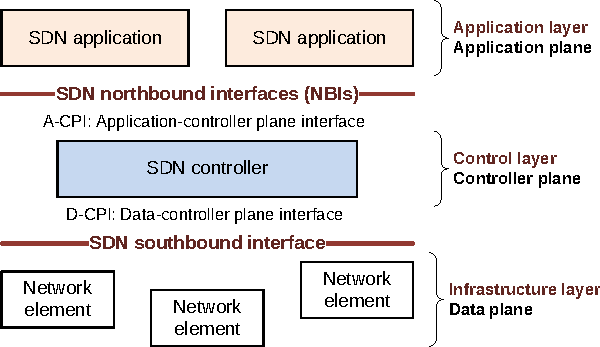
\includegraphics[width=.6\linewidth]{img/sdn_basic_schema.pdf}
    \caption{A schema of basic SDN components.}
    \label{fig:sdn-schema}
\end{figure}

\emph{Software-defined networking} is a loosely defined concept of separating the networking data plane (infrastructure layer) and the control plane (control layer) into separate components. In traditional networking architectures, each network device makes forwarding and/or routing decisions fully autonomously. SDNs separate the decision-making and data processing into distinct layers (see \cref{fig:sdn-schema}) and define two main interfaces. \emph{SDN applications} provide the \emph{SDN controller} with networking requirements using the \emph{northbound interface}. The controller then configures the actual network equipment using the \emph{southbound interface}.

\emph{OpenFlow}\footnote{\url{https://opennetworking.org/sdn-resources/openflow-switch-specification/}} is a de-facto standard protocol for the southbound interface. \emph{Container network interface (CNI)} is a specification for the northbound interface in Kubernetes and other container orchestrators.

\section{OpenFlow}

\todo{add a proper example to the table}

\emph{OpenFlow} is a protocol for configuring packet forwarders (generalized switches). The forwarding tables (see \cref{tab:openflow-forwarding-table}) in the network switches are filled with rules provided by the OpenFlow controller. The flow rules consist of two parts:

\begin{itemize}
    \item \emph{Packet matching criteria} which can include value masks for not only Ethernet header values, but also IP, transport layer protocols (TCP, UDP, ...), and more depending on the version of the OpenFlow protocol. 
    \item The action instructing the switch on what to do with the matching packets. Possible actions include dropping packets, modifying header fields, forwarding to physical or virtual ports, sending to the controller, and more.
\end{itemize}

In addition to the externally configured flow rules, the forwarding tables also contain statistics updated every time the flow rule is used. The OpenFlow controller can then query switches for these statistics.

\begin{table}[]
    \begin{center}
        \caption{Schema of an OpenFlow forwarding table}
        \label{tab:openflow-forwarding-table}
        \begin{tabular}{c|c|c}
            \textbf{Matching criteria} & \textbf{Action} & \textbf{Statistics} \\
            \hline
            \xxx{add example} & 1110.1 & a\\ % <--
            2 & 10.1 & b\\ % <--
            3 & 23.113231 & c\\ % <--
        \end{tabular}
    \end{center}
\end{table}


\section{Open vSwitch}

\emph{Open vSwitch} (OVS) is a multilayer virtual switch. OVS runs as a software switch on all major platforms and supports hardware offload for its data processing layers. The supported OpenFlow protocol allows any SDNs to use OVS in its infrastructure layer.

The internal architecture of OVS mirrors the SDN architecture (see \cref{fig:ovs-arch-schema}\todo{redraw the image or quote it properly}). \ident{ovs-vswitchd} (or just \ident{vswitchd}) is the OVS's control process. \ident{vswitchd} communicates via the OpenFlow protocol and stores the configured flow rules in a purpose-built Open vSwitch Database (OVSDB). Alternatively, the database can be accessed externally, and OVS can be configured without using the OpenFlow wire protocol.

A \emph{datapath} is the lowest component of OVS physically forwarding packets between configured ports. There are multiple datapath implementations, some of them implemented fully in the \ident{vswitchd} process, some of them using extra kernel modules for improved performance. \ident{vswitchd} translates the OpenFlow flow rules into a more efficient and simplified form. These simplified flow rules are then used by the datapaths to make forwarding decisions.

\begin{table}[h!]
    \begin{center}
        \caption{Overview of OVS components}
        \label{tab:ovs-components}
        \begin{tabular}{p{0.2\linewidth}|p{0.7\linewidth}}
            \textbf{Component} & \textbf{Description} \\
            \hline
            % FIXME this footnote might be on a wrong page :(
            \ident{ovsdb}\tablefootnote{\url{https://docs.openvswitch.org/en/latest/ref/ovsdb.7/}} & OVSDB instance storing the OpenFlow flow rules \\
            \hline
            \ident{ovs-vswitchd}\tablefootnote{\url{http://www.openvswitch.org/support/dist-docs/ovs-vswitchd.8.html}} & a process managing datapaths and providing OpenFlow configuration interface \\
            \hline
            datapath & a logical component in \ident{ovs-vswitchd}, does the actual packet forwarding \\
        \end{tabular}
    \end{center}
\end{table}


\section{Open Virtual Network}

\todo{link to documentation \url{https://access.redhat.com/documentation/en-us/red_hat_openstack_platform/13/html/networking_with_open_virtual_network/open_virtual_network_ovn}}

\emph{Open Virtual Network} (OVN) is an SDN combining Open vSwitch with network tunnels (by default GENEVE) for its infrastructure layer. Applications communicate with OVN through the \ident{northdb}, an OVSDB instance storing high-level network configuration in terms of traditional networking concepts. The \ident{ovn-northd} process translates the configuration into logical datapath flows and stores the result in the \ident{southdb} OVSDB instance. The \ident{ovn-controller} then distributes the flows from the \ident{southdb} into individual OVS databases.

\begin{table}[h!]
    \begin{center}
        \caption{Overview of OVN components}
        \label{tab:ovn-components}
        \begin{tabular}{p{0.23\linewidth}|p{0.47\linewidth}|p{0.2\linewidth}}
            \textbf{Component} & \textbf{Description} & \textbf{How it runs} \\
            \hline
            \ident{northdb} & OVSDB instance storing network configuration in terms of traditional networking concepts & centralized or distributed \\
            \hline
            \ident{ovn-northd} & process translating configuration into logical flows & centralized or distributed \\
            \hline
            \ident{southdb} & OVSDB instance storing network configuration in terms of logical flows & centralized or distributed\\
            \hline
            \ident{ovn-controller} & configures local OVS from the \ident{southdb} & locally on every node\\
        \end{tabular}
    \end{center}
\end{table}


\section{OVN-Kubernetes}

\emph{OVN-Kubernetes}\footnote{\url{https://github.com/ovn-org/ovn-kubernetes}} is a Kubernetes CNI plugin using OVN in the background. \todo{Expand with information about internal architecture.}

\section{Open vSwitch Datapath Internals}
\label{sec:ovs-packet-processing}
\todo{This whole section is not adapted to the thesis yet. It is just copy-pasted from my website.}

\begin{figure}
    \centering
    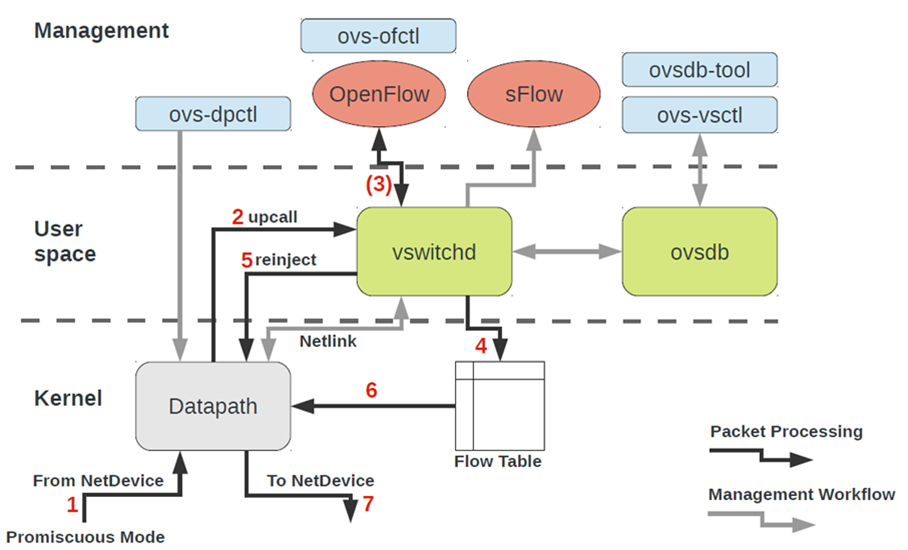
\includegraphics[width=.9\linewidth]{img/ovs_architecture_01.png}
    \caption{Schema of OVS internal architecture.}
    \label{fig:ovs-arch-schema}
\end{figure}

\ident{ovs-vswitchd} processes packets in \href{https://github.com/openvswitch/ovs/blob/e90a0727f17f6ad915a32735a8c0b282f2c8cd6f/lib/dpif.h}{datapaths}, which is essentially \href{https://github.com/openvswitch/ovs/blob/e90a0727f17f6ad915a32735a8c0b282f2c8cd6f/lib/dpif-provider.h\#L107-L117}{an interface} hiding the implementation details of low-level packet processing. The datapath does not do any decisions by itself, it's the clients of the datapath that tell it what to do by giving it simple rules to follow. In the upstream code, there are two datapath implementations - \href{https://github.com/openvswitch/ovs/blob/e90a0727f17f6ad915a32735a8c0b282f2c8cd6f/lib/dpif-netdev.c}{\ident{netdev}} and \href{https://github.com/openvswitch/ovs/blob/e90a0727f17f6ad915a32735a8c0b282f2c8cd6f/lib/dpif-netlink.c}{\ident{netlink}}.

The \ident{netdev} datapath is implemented entirely in user space, and it's multiplatform. All major operating systems are currently supported. As it's userspace only, it's less performant than the \ident{netlink} datapath and we will ignore it for the rest of this article. The \ident{netlink} datapath is Linux-specific. It resides partially in a kernel module and partially in user space. The kernel module does most of the packet processing. The userspace communicates with the kernel over a netlink socket, exchanging commands and packets. Most packets never touch the user space and are processed only in the kernel. We call this the fast-path. The alternative is the slow-path, a path through user space, which is taken every time the fast-path fails.


\subsection{Overview of the kernel and user space interactions}
\label{overview-of-the-kernel-and-user-space-interactions}

The fast-path involves matching incoming packet against a set of flow rules stored in the kernel. The rules contain actions -- instructions describing what to do next with the packet. If any of the flow rules matches, the kernel blindly executes the action. In this case, no buffering is involved, the packets are processed immediately.

The slow-path gets involved when the fast-path fails (no flow rule match) or when the action in the flow rule asks for it. In it, the packet is passed to the user-space via a netlink socket (we call this an upcall). An user-space process receives the packet, processes it according to its configuration and reinjects it back into the kernel. Additionally, a new flow rule can be installed into the kernel to speed up future processing of similar packets. The slow-path buffers packets when they are passed from kernel to user-space.

\subsection{The fast-path}
\label{the-fast-path}

\subsubsection{The data structures}
\label{the-data-structures}

The flow table (\href{https://elixir.bootlin.com/linux/v6.2.6/source/net/openvswitch/flow_table.h\#L62}{\ident{struct\ flow\_table}}) is an in-kernel data structure, which stores flows rules (\href{https://elixir.bootlin.com/linux/v6.2.6/source/net/openvswitch/flow.h\#L221}{\ident{struct\ sw\_flow}}) and allows for fast matching with individual packets. Every flow also contains a list of actions (\href{https://elixir.bootlin.com/linux/v6.2.6/source/net/openvswitch/flow.h\#L206}{\ident{struct\ sw\_flow\_actions}}).

Every flow has a flow key (\href{https://elixir.bootlin.com/linux/v6.2.6/source/net/openvswitch/flow.h\#L75}{\ident{struct\ sw\_flow\_key}}) and a bitmask (\href{https://elixir.bootlin.com/linux/v6.2.6/source/net/openvswitch/flow.h\#L183}{\ident{struct\ sw\_flow\_mask}}). The combination of both of these enables the packet matching. The key is a complex structure with parsed out packet header values. It can be created from any Ethernet frame (\href{https://elixir.bootlin.com/linux/v6.2.6/source/net/openvswitch/flow.c\#L886}{\ident{key\_extract}}). The mask then tells us which bits between the extracted packet key and the flow key must match.


\subsubsection{The matching algorithm}
\label{the-matching-algorithm}

When processing a packet, we create the corresponding flow key and look for matching flows in the flow table. The packet can match any number of flows, but we always use the first one we find. The userspace component is made responsible for preventing overlapping conflicting flow rules.

The flow table stores the flow in a hash table, where the key is the masked \ident{sw\_flow\_key}. Therefore, to find a flow for a packet, we must try several masks. The lookup procedure could look like this:

\begin{verbatim}
    def lookup(flow_table, key):
        for mask in flow_table.mask_array:
            masked_key = apply mask to key
            if masked_key in flow_table.flows:
                return flow_table.flows[masked_key]
        return None
\end{verbatim}
    

The real implementation (\href{https://elixir.bootlin.com/linux/v6.2.5/source/net/openvswitch/flow_table.c\#L785}{\ident{ovs\_flow\_tbl\_lookup\_stats}}) is in principle similar, but more optimized:

\begin{enumerate}
\def\labelenumi{\arabic{enumi}.}
\item
  The kernel keeps mask usage statistics and the \ident{mask\_array} is
  kept sorted with the most used masks first
  (\href{https://elixir.bootlin.com/linux/v6.2.5/source/net/openvswitch/flow_table.c\#L1107}{\ident{ovs\_flow\_masks\_rebalance}}).
  This happens
  \href{https://elixir.bootlin.com/linux/v6.2.5/source/net/openvswitch/datapath.c\#L2536}{periodically}
  based on a time interval.
\item
  There is already a \ident{sk\_buff}
  \href{https://elixir.bootlin.com/linux/v6.2.5/source/include/linux/skbuff.h\#L1537}{hash}
  based on source/destination addresses and ports. The lookup procedure
  makes use of the hash by having a fixed size
  (\href{https://elixir.bootlin.com/linux/v6.2.5/source/net/openvswitch/flow_table.c\#L41}{256})
  hash table storing references to their masks. The cached masks are
  then tried first. If there is no match, standard lookup over all masks
  follows. This helps with burst performance.
\end{enumerate}

\subsection{The slow-path}
\label{the-slow-path}

The user space process (\href{https://www.man7.org/linux/man-pages/man8/ovs-vswitchd.8.html}{\ident{ovs-vswitchd}}) communicates with the kernel over netlink socket. When packet leaves the
fast-path, it is temporarily buffered in a queue (\href{https://elixir.bootlin.com/linux/v6.2.6/source/net/openvswitch/datapath.c\#L311}{\ident{ovs\_dp\_upcall}}) when crossing the kernel boundary.

\ident{ovs-vswitchd} reads packets from the kernel in several threads. The datapath interface defines a \href{https://github.com/openvswitch/ovs/blob/e90a0727f17f6ad915a32735a8c0b282f2c8cd6f/lib/dpif-provider.h\#L387-L408}{\ident{recv}} function for receiving a single packet from the kernel. The netlink datapath implements it with the function \href{https://github.com/openvswitch/ovs/blob/e90a0727f17f6ad915a32735a8c0b282f2c8cd6f/lib/dpif-netlink.c\#L3132-L3134}{\ident{dpif\_netlink\_recv}}.

Higher up, the \ident{recv} datapath interface function is used in generic \href{https://github.com/openvswitch/ovs/blob/e90a0727f17f6ad915a32735a8c0b282f2c8cd6f/lib/dpif.c\#L1591-L1611}{\ident{dpif\_recv}} which also provides an useful tracepoint \href{https://github.com/openvswitch/ovs/blob/e90a0727f17f6ad915a32735a8c0b282f2c8cd6f/lib/dpif.c\#L1618}{\ident{dpif\_recv\_\_recv\_upcall}} for measurements. Even higher up the abstraction stack, the function \href{https://github.com/openvswitch/ovs/blob/e90a0727f17f6ad915a32735a8c0b282f2c8cd6f/ofproto/ofproto-dpif-upcall.c\#L829-L830}{\ident{recv\_upcalls}} in the file \ident{ofproto-dpif-upcall.c} reads packets in batches, which are then processed by \href{https://github.com/openvswitch/ovs/blob/e90a0727f17f6ad915a32735a8c0b282f2c8cd6f/ofproto/ofproto-dpif-upcall.c\#L1639-L1641}{\ident{handle\_upcalls}}. The \ident{handle\_upcalls} function essentially transforms the list of packets into a list of operations that should be executed on the datapath. This includes adding new flows to the datapath as well as simply sending packets where they belong.

Parallel with upcall processing, OVS also runs several maintenance tasks. A \href{https://github.com/openvswitch/ovs/blob/e90a0727f17f6ad915a32735a8c0b282f2c8cd6f/ofproto/ofproto-dpif-upcall.c\#L3312-L3336}{balancing task} makes sure, that when the system is under stress, the most used flow rules are in the kernel. \href{https://github.com/openvswitch/ovs/blob/e90a0727f17f6ad915a32735a8c0b282f2c8cd6f/ofproto/ofproto-dpif-upcall.c\#L83-L111}{A revalidator task} periodically reads statistics from the kernel and most importantly, removes old unused flows.

% TODO add sources
%
% \begin{center}\rule{0.5\linewidth}{0.5pt}\end{center}
% 
% \hypertarget{sources}{%
% \section{Sources}\label{sources}}
% 
% \begin{itemize}
% \tightlist
% \item
%   \href{https://docs.openvswitch.org/en/latest/contents/}{Open vSwitch
%   online documentation}
% 
%   \begin{itemize}
%   \tightlist
%   \item
%     \href{https://docs.openvswitch.org/en/latest/topics/datapath/}{Open
%     vSwitch Datapath Development Guide}
%   \end{itemize}
% \item
%   \href{https://elixir.bootlin.com/linux/v6.2.6/source}{Linux Kernel
%   source code}
% \item
%   \href{https://github.com/openvswitch/ovs/tree/51778134d4c8a84801230b1e5a7d59e180d9e8b5}{Open
%   vSwitch source code}
% \item
%   \href{https://developers.redhat.com/articles/2022/02/07/investigating-cost-open-vswitch-upcalls-linux}{RedHat
%   Developer Blog: Investigating the cost of Open vSwitch upcalls in
%   Linux}
% \item
%   \href{https://hustcat.github.io/an-introduction-to-ovs-architecture/}{An
%   introduction to OVS architecture}
% \end{itemize}
\chapter{Experimental environment}
\label{chap:env}

This chapter describes the environment we used for running our experiments. The information provided here should allow anyone to replicate our measurements.

\section{Hardware}
\label{sec:hw-env}

For our research, we used two experimental cluster with different hardware configurations. One installation run virtualized on Proxmox VE with only a single physical host. The other installation used dedicated hardware. When we write about an experiment and do not specify where it runs, we are presenting results from the cluster on dedicated hardware. However, most of the measurements can be replicated in a virtualized environment without a significant impact on the outcome.

\paragraph{Virtualized installation}
We used the virtualized environment for development and debugging. The physical host was running Proxmox VE 7.4-3, and it was configured with an Intel\textsuperscript{\textregistered} Core\textsuperscript{TM} i7-3770 CPU running at 3.40 GHz with $4$ cores, $8$ threads, and $31.23$ GiB of RAM.

The virtual machines used for the cluster nodes were each configured with $4$ virtual cores and $4$ GiB of RAM. We had initially started experimenting with $2$ CPU cores per node to prevent overprovisioning, but our workloads always fully stressed only one node (always \kb{2}), and we were mostly interested in system behavior with multiple threads. The overprovisioning did not seem to cause any problems.

The cluster nodes were equipped with $2$ virtual network interfaces connected to two virtual Linux bridges on the host. We used one interface for system management and WAN access. Tthe other bridge was used for cluster interconnect. We did not artificially limit the throughput or latency of the link between nodes. When measured between \kb{2} and \kb{3} using \ident{iperf3} with the default configuration and \ident{ping} with $100$ samples, the throughput was $14.5$ Gbps and the average round trip time $0.383$ ms.

\paragraph{Dedicated hardware}

We used the cluster with dedicated hardware to validate the results observed in the virtual environment. The nodes were Dell PowerEdge R730 servers, configured with Intel\textsuperscript{\textregistered} Xeon\textsuperscript{\textregistered} CPU E5-2690 v4 running at 2.60GHz with $14$ cores, $28$ threads, and $131$ GB of RAM.

Similar to the virtualized nodes, the dedicated nodes had 2 network interfaces. One management 1 GbE interface was connected to the Internet, and another cluster only 10 GbE interface was connected to a switch. We configured the switch to use VLANs to isolate the cluster traffic from all other ports. While we did not have the opportunity to use a fully dedicated switch, the switch should have had enough capacity that it would not be a bottleneck. The average round trip time between \kb{2} and \kb{3} (\ident{ping -c 100}) was $0.104$ ms.

\section{Software environment}
\label{sec:sw-env}

We run our experiments and measurements on a Kubernetes cluster with OVN-Kubernetes as the CNI plugin and Docker as the container runtime. OVN-Kubernetes was installed using containerized setup following the official installation guide \cite{OVNInstallGuide}. We used Fedora 38 as the base Linux distribution. To allow reproducibility, we fully automated the installation procedure. Installation scripts with usage instructions can be found in \cref{chap:install}.

In our experiments, we always used a three-node cluster with one node dedicated as a control node. We didn't test cluster installations configured for high availability (HA). We focused on the internals of OVS, a part of low-level networking infrastructure. We do not expect any significant difference between HA and non-HA clusters.

We named our cluster nodes \kb{1}, \kb{2}, and \kb{3}. The node \kb{1} is always the control node, our experiments always run on \kb{2}.

\subsection{OVN-Kubernetes configuration}
\label{subsec:ovnkube-limits}

We deployed a fully containerized OVN-Kubernetes, meaning that even OVS was deployed in a privileged container. The default OVS container spec file contains \href{https://github.com/ovn-org/ovn-kubernetes/blob/master/dist/templates/ovs-node.yaml.j2\#L84-L90}{this resource limit}:

\begin{verbatim}
resources:
    requests:
        cpu: 100m
        memory: 300Mi
    limits:
        cpu: 200m
        memory: 400Mi
\end{verbatim}

We have manually removed this limit for most of our experiments. We have also tested with the limit active and we always explicitly mention it when it is the case.

\subsection{OVS modifications}

Instead of the default OVS container, we configured our systems with a modified version to improve observability. Our changes included:

\begin{itemize}
    \item We added development tools (e.g. \ident{gdb}, \ident{perf}, ...) to the container image.
    \item We recompiled \ident{ovs-vswitchd} to include additional user statically-defined tracing (USDT) \cite{USDT} probes
    \item We included debug symbols in the \ident{ovs-vswitchd} executable
\end{itemize}

Implementation details and instructions on how to replicate our build are in \cref{chap:ovs-mod}.

\subsection{Kubernetes configuration}

We always deployed three different pods to the Kubernetes cluster. The spec files are attached to this work. The pods were:

\begin{itemize}
    \item \ident{arch} on \kb{2} -- a pod running the latest Arch Linux Docker image. We used this pod for the main part of our experiments.

    \item \ident{victim} on \kb{2} -- again, a pod with the latest Arch Linux image. We used it to measure the impact of our experiments on pods sharing the same node.

    \item \ident{reflector} on \kb{3} -- a privileged Arch Linux container with a custom raw-socket-based packet reflector and \ident{iptables} rule preventing the kernel from sending ICMP connection refused packets. The reflector swapped the Ethernet and IP addresses in the received packets and sent them out again.
\end{itemize}

\subsection{Experiment implementation}

We developed our experiments mainly in Rust. Everything is contained within one project in a tool we call the \ident{analyzer}. In the few cases when Rust was not the best language for the task, we embedded scripts in other languages (mainly Bash and Python) in the Rust executable itself. Our Rust code always provides an entry point.

The main reasoning behind the language and architecture choice was personal preferences and ease of distribution -- the ability to create a single statically-linked executable that would work almost anywhere.

Implementation details and usage instructions are in \cref{chap:analyzer}.

\subsection{Clock synchronization}

All our experiments use Linux's \ident{CLOCK\_MONOTONIC} clock for timekeeping. Because we measure everything on a single node, \kb{2}, the clock is perfectly consistent across different containers. There could be small discrepancies due to synchronization between CPU cores and scheduling, but we are mostly concerned about larger time scales so we assume these discrepancies will not affect our results.


\chapter{Experiment design}
\label{chap:design}

As we showed in \cref{chap:refs}, OVS inserts flow rules into datapaths on demand after upcalls. Therefore, some packets require much more processing and can slow the system down. Eelco Chaudron investigated the cost of an upcall in OVS\todo{link source} using eBPF probes in the Linux kernel. His experiments show that processing a packet through the slow path can take anywhere between \qty{700}{\us} and \qty{10}{\ms} extra compared to the fast path.

Based on this knowledge, we tried to answer the following questions about OVS internals:

\begin{itemize}
    \item When are flow rules removed from the datapaths? (\cref{design:flow-eviction})
    \item What is the cost of an upcall when measured from the user space? (\cref{design:upcall-cost})
    \item Which packets generate upcalls? (\cref{design:upcall-generators})
    \item What is the impact of artificial upcall-only traffic on the performance of the whole system? (\cref{design:upcall-impact})
\end{itemize}

The following sections describe our methods to answer the questions. The next chapter discusses our results.


% quote https://developers.redhat.com/articles/2022/02/07/investigating-cost-open-vswitch-upcalls-linux


\section{Removal of flow rules from datapaths}
\label{design:flow-eviction}

We can observe an effect of an upcall using the \ident{ping} tool. The first packet has higher latency than the rest of the ICMP packets.

\vspace{0.5cm}

\begin{lstlisting}[caption=Output of the \ident{ping} command in the virtualized environment, captionpos=b, basicstyle=\ttfamily\scriptsize]
[root@kb2 ~]# ping -c 5 kb3
PING kb3 (192.168.1.223) 56(84) bytes of data.
64 bytes from kb3 (192.168.1.223): icmp_seq=1 ttl=64 time=1.19 ms
64 bytes from kb3 (192.168.1.223): icmp_seq=2 ttl=64 time=0.404 ms
64 bytes from kb3 (192.168.1.223): icmp_seq=3 ttl=64 time=0.365 ms
64 bytes from kb3 (192.168.1.223): icmp_seq=4 ttl=64 time=0.424 ms
64 bytes from kb3 (192.168.1.223): icmp_seq=5 ttl=64 time=0.304 ms

--- kb3 ping statistics ---
5 packets transmitted, 5 received, 0% packet loss, time 4062ms
rtt min/avg/max/mdev = 0.304/0.536/1.185/0.326 ms
\end{lstlisting}

The first packet delay is absent when we run the \ident{ping} command for the second time shortly after the first. The higher latency is visible again. This behavior can be explained by a flow rule eviction timeout that removes the rule from the datapath's forwarding table.

Assuming the timeout stays constant, we can measure it by varying the interval between ICMP packets. The dependency between the measured latency and the time delay should be constant except for one sharp increase in latency when the delays get longer than the timeout.

\paragraph{Our experiment}
We conducted the experiment in the following way:

\begin{enumerate}
    \item Generate a random number $D$ in the interval $\interval{8}{12}$
    \item sleep for $D$ seconds
    \item run \ident{ping -c 2 192.168.1.221}
    \item log $D$ and both round trip times
    \item goto step 1 until we have enough
\end{enumerate}

We chose the interval based on non-rigorous preliminary experiments. After plotting RTT's dependence on the delay $D$, we expect to see:

\begin{itemize}
    \item The first RTT data points will form a line with a sharp increase at a value of $D$ corresponding to the eviction timeout

    \item The second RTT data points will form only a single horizontal line.
\end{itemize}

Results of this experiment can be found in \cref{res:eviction-timeout}.

\section{Cost of an upcall}
\label{design:upcall-cost}

Eelco Chaudron's research into the cost of an upcall used eBPF to measure upcall cost directly in the kernel. However, as we saw in the previous section, upcalls have visible effects outside of the kernel.

The unchanged experiment devised in the previous section provides us with a direct measurement of the observable upcall effect. In each data point, we can subtract the two round-trip-times to get an insight into how much time upcall costs.

While this measurement methodology leads to less precise results than when directly measuring the in-kernel execution time using eBPF, we can use it to measure the upcall cost without special privileges on publicly deployed cloud hosting services.\todo{má smysl tohle zmiňovat, když to nezkusím? Napsal jsem do MetaCentra a domluvili jsme se, ze se mi ozvou. Ale zatim nic.}

Our results can be found in \cref{res:upcall-cost}.

\section{Packets generating upcalls}
\label{design:upcall-generators}

To stress-test the slow path, we have to be able to generate upcalls consistently. We have to find types of packets that will repeatedly miss all installed flow rules in the OVS datapath. We have a choice between a static analysis and a dynamic analysis of OVS.

We chose to approach the problem using dynamic analysis. We decided on dynamic analysis instead of static analysis because the results depend on OVS, the whole SDN, and its configuration. For static analysis, the search space is just too large. Also, the dynamic analysis tooling can be later reused on different OVS deployment than ours.

Our experiment sends varying packets in batches based on their type and monitors the upcalls and flow table changes using kprobes in the kernel and user statically-defined tracing (USDT) probes in \ident{ovs-vswitchd}.

The flow rules in OVS datapaths use the \ident{struct sw\_flow\_key}\todo{link} to represent the flow key. For every field of that structure, our measurement tool sends 1000 packets with the corresponding packet header field randomized and everything else fixed at arbitrary values.

We used Scapy to generate the packets. For example, the code to generate random TTL values in an IPv4 packet looks like this:

\begin{verbatim}
tag("IP(ttl)")
sendp(Ether(dst="aa:bb:cc:dd:ee:ff") / IP(dst="10.244.1.1", ttl=RandByte()), count=1000)
sleep(11)  # more than the eviction timeout
\end{verbatim}

Because we used dynamic analysis, we can not be certain that we covered all possible cases. We can draw some general conclusions from the measurement results and look into the source code for additional insights. However, there is always the possibility that we missed something.

\section{Impact of upcall-only traffic}
\label{design:upcall-impact}

\paragraph{Stress testing tool}
From the previous experiment, we learned that randomized unicast Ethernet source addresses generate upcalls. We used this knowledge to write a custom tool for sending minimalistic Ethernet frames. The Ethernet header needs only 14 bytes, but we used 16-byte packets due to slightly better performance. Instead of randomization, we filled the source Ethernet addresses with an increasing integer sequence.

Our tool is optimized for controlled and regular packet generation. Configured with a time interval between packets or a desired packet frequency, it tries to send packets as regularly as possible:

\begin{verbatim}
start_time = clock()
sent = 0
while True:
    now = clock()
    while we should have sent more packets than we sent:
        sent a new packet
        sent += 1
    
    sleep( until next packet is scheduled )
\end{verbatim}

Only instead of sending the packets one by one every time, we send them in batches using \ident{io\_uring} if it is possible. When we set the interval to \qty{1}{\ns} (zero is not possible due to division by zero), we can reach roughly 210k packets per second in a single thread on the dedicated test server.

\paragraph{The experiment}
For our experiment, we stressed OVS using our tool and monitored the system. We mainly measured OVS's memory consumption, the load average of the whole system and latencies observable from the \ident{victim} pod.

The results of the experiment can be found in \cref{res:upcall-stress}.

\chapwithtoc{Conclusion}

In the conclusion, you should summarize what was achieved by the thesis. In a few paragraphs, try to answer the following:
\begin{itemize}
\item Was the problem stated in the introduction solved? (Ideally include a list of successfully achieved goals.)
\item What is the quality of the result? Is the problem solved for good and the mankind does not need to ever think about it again, or just partially improved upon? (Is the incompleteness caused by overwhelming problem complexity that would be out of thesis scope\todo{This is quite common.}, or any theoretical reasons, such as computational hardness?)
\item Does the result have any practical applications that improve upon something realistic?
\item Is there any good future development or research direction that could further improve the results of this thesis? (This is often summarized in a separate subsection called `Future work'.)
\end{itemize}


\ifEN
\chapwithtoc{Bibliography}
\else
\chapwithtoc{Seznam použité literatury}
\fi

\printbibliography[heading=none]


\appendix
\chapter{Using CoolThesisSoftware}

Use this appendix to tell the readers (specifically the reviewer) how to use your software. A very reduced example follows; expand as necessary. Description of the program usage (e.g., how to process some example data) should be included as well.

To compile and run the software, you need dependencies XXX and YYY and a C compiler. On Debian-based Linux systems (such as Ubuntu), you may install these dependencies with APT:
\begin{Verbatim}
apt-get install \
  libsuperdependency-dev \
  libanotherdependency-dev \
  build-essential
\end{Verbatim}

To unpack and compile the software, proceed as follows:
\begin{Verbatim}
unzip coolsoft.zip
cd coolsoft
./configure
make
\end{Verbatim}

The program can be used as a C++ library, the simplest use is demonstrated in \cref{lst:ex}. A demonstration program that processes demonstration data is available in directory \verb|demo/|, you can run the program on a demonstration dataset as follows:
\begin{Verbatim}
cd demo/
./bin/cool_process_data data/demo1
\end{Verbatim}

After the program starts, control the data avenger with standard \verb-WSAD- controls.

\begin{listing}
\begin{lstlisting}
#include <CoolSoft.h>
#include <iostream>

int main() {
	int i;
	if(i = cool::ProcessAllData()) // returns 0 on error
		std::cout << i << std::endl;
	else
		std::cerr << "error!" << std::endl;
	return 0;
}
\end{lstlisting}
\caption{Example program.}
\label{lst:ex}
\end{listing}


% if your attachments are complicated, describe them in a separate appendix
%\include{attachments}

\openright
\end{document}
